% appendix/questions/questions.tex

\QuickQuizChapter{cha:app:Important Questions}{Important Questions}

\epigraph{Ask me no questions, and I'll tell you no fibs.}
	 {\emph{``She Stoops to Conquer'', Oliver Goldsmith}}

The following sections discuss some important questions relating to
SMP programming.
Each section also shows how to {\em avoid} having to worry about
the corresponding question, which can be extremely important if
your goal is to simply get your SMP code working as quickly and
painlessly as possible --- which is an excellent goal, by the way!

Although the answers to these questions are often quite a bit less
intuitive than they would be in a single-threaded setting,
with a bit of work, they are not that difficult to understand.
If you managed to master recursion, there is nothing in here that should
pose an overwhelming challenge.

% @@@ roadmap...

% @@@ doesn't parallel automatically make things faster? (locked increment)
% @@@ doesn't getting rid of locks get rid of all these problems? (atomic inc)
% @@@ doesn't NBS take care of all these problems? (cite IPDPS paper)

% appendix/questions/after.tex

\section{What Does ``After'' Mean?}
\label{sec:app:questions:What Does ``After'' Mean?}

``After'' is an intuitive, but surprisingly difficult concept.
An important non-intuitive issue is that code can be delayed at
any point for any amount of time.
Consider a producing and a consuming thread that communicate using
a global struct with a timestamp ``t'' and integer fields ``a'', ``b'',
and ``c''.
The producer loops recording the current time
(in seconds since 1970 in decimal),
then updating the values of ``a'', ``b'', and ``c'',
as shown in Figure~\ref{fig:app:questions:After Producer Function}.
The consumer code loops, also recording the current time, but also
copying the producer's timestamp along with the fields ``a'',
``b'', and ``c'', as shown in
Figure~\ref{fig:app:questions:After Consumer Function}.
At the end of the run, the consumer outputs a list of anomalous recordings,
e.g., where time has appeared to go backwards.

\begin{figure}[htbp]
{ \scriptsize
\begin{verbatim}
  1 /* WARNING: BUGGY CODE. */
  2 void *producer(void *ignored)
  3 {
  4   int i = 0;
  5
  6   producer_ready = 1;
  7   while (!goflag)
  8     sched_yield();
  9   while (goflag) {
 10     ss.t = dgettimeofday();
 11     ss.a = ss.c + 1;
 12     ss.b = ss.a + 1;
 13     ss.c = ss.b + 1;
 14     i++;
 15   }
 16   printf("producer exiting: %d samples\n", i);
 17   producer_done = 1;
 18   return (NULL);
 19 }
\end{verbatim}
}
\caption{``After'' Producer Function}
\label{fig:app:questions:After Producer Function}
\end{figure}

\begin{figure}[htbp]
{ \scriptsize
\begin{verbatim}
  1 /* WARNING: BUGGY CODE. */
  2 void *consumer(void *ignored)
  3 {
  4   struct snapshot_consumer curssc;
  5   int i = 0;
  6   int j = 0;
  7
  8   consumer_ready = 1;
  9   while (ss.t == 0.0) {
 10     sched_yield();
 11   }
 12   while (goflag) {
 13     curssc.tc = dgettimeofday();
 14     curssc.t = ss.t;
 15     curssc.a = ss.a;
 16     curssc.b = ss.b;
 17     curssc.c = ss.c;
 18     curssc.sequence = curseq;
 19     curssc.iserror = 0;
 20     if ((curssc.t > curssc.tc) ||
 21         modgreater(ssc[i].a, curssc.a) ||
 22         modgreater(ssc[i].b, curssc.b) ||
 23         modgreater(ssc[i].c, curssc.c) ||
 24         modgreater(curssc.a, ssc[i].a + maxdelta) ||
 25         modgreater(curssc.b, ssc[i].b + maxdelta) ||
 26         modgreater(curssc.c, ssc[i].c + maxdelta)) {
 27       i++;
 28       curssc.iserror = 1;
 29     } else if (ssc[i].iserror)
 30       i++;
 31     ssc[i] = curssc;
 32     curseq++;
 33     if (i + 1 >= NSNAPS)
 34       break;
 35   }
 36   printf("consumer exited, collected %d items of %d\n",
 37          i, curseq);
 38   if (ssc[0].iserror)
 39     printf("0/%d: %.6f %.6f (%.3f) %d %d %d\n",
 40            ssc[0].sequence, ssc[j].t, ssc[j].tc,
 41            (ssc[j].tc - ssc[j].t) * 1000000,
 42            ssc[j].a, ssc[j].b, ssc[j].c);
 43   for (j = 0; j <= i; j++)
 44     if (ssc[j].iserror)
 45       printf("%d: %.6f (%.3f) %d %d %d\n",
 46              ssc[j].sequence,
 47              ssc[j].t, (ssc[j].tc - ssc[j].t) * 1000000,
 48              ssc[j].a - ssc[j - 1].a,
 49              ssc[j].b - ssc[j - 1].b,
 50              ssc[j].c - ssc[j - 1].c);
 51   consumer_done = 1;
 52 }
\end{verbatim}
}
\caption{``After'' Consumer Function}
\label{fig:app:questions:After Consumer Function}
\end{figure}

\QuickQuiz{}
	What SMP coding errors can you see in these examples?
	See \url{time.c} for full code.
\QuickQuizAnswer{
	\begin{enumerate}
	\item	Missing barrier() or volatile on tight loops.
	\item	Missing Memory barriers on update side.
	\item	Lack of synchronization between producer and consumer.
	\end{enumerate}
} \QuickQuizEnd

One might intuitively expect that the difference between the producer
and consumer timestamps would be quite small, as it should not take
much time for the producer to record the timestamps or the values.
An excerpt of some sample output on a dual-core 1GHz x86 is shown in
Table~\ref{fig:app:questions:After Program Sample Output}.
Here, the ``seq'' column is the number of times through the loop,
the ``time'' column is the time of the anomaly in seconds, the ``delta''
column is the number of seconds the consumer's timestamp follows that
of the producer (where a negative value indicates that the consumer
has collected its timestamp before the producer did), and the
columns labelled ``a'', ``b'', and ``c'' show the amount that these
variables increased since the prior snapshot collected by the consumer.

\begin{table}[htbp]
{ \scriptsize
\begin{tabular}{rcrrrr}
seq    & time (seconds) & delta~    &  a &  b &  c \\
\hline
17563: & 1152396.251585 & (-16.928) & 27 & 27 & 27 \\
18004: & 1152396.252581 & (-12.875) & 24 & 24 & 24 \\
18163: & 1152396.252955 & (-19.073) & 18 & 18 & 18 \\
18765: & 1152396.254449 & (-148.773) & 216 & 216 & 216 \\
19863: & 1152396.256960 & (-6.914) & 18 & 18 & 18 \\
21644: & 1152396.260959 & (-5.960) & 18 & 18 & 18 \\
23408: & 1152396.264957 & (-20.027) & 15 & 15 & 15 \\
\end{tabular}
}
\caption{``After'' Program Sample Output}
\label{fig:app:questions:After Program Sample Output}
\end{table}

Why is time going backwards?
The number in parentheses is the difference in microseconds, with
a large number exceeding 10 microseconds, and one exceeding even
100 microseconds!
Please note that this CPU can potentially execute about more than 100,000
instructions in that time.

One possible reason is given by the following sequence of events:
\begin{enumerate}
\item	Consumer obtains timestamp
	(Figure~\ref{fig:app:questions:After Consumer Function}, line 13).
\item	Consumer is preempted.
\item	An arbitrary amount of time passes.
\item	Producer obtains timestamp
	(Figure~\ref{fig:app:questions:After Producer Function}, line 10).
\item	Consumer starts running again, and picks up the consumer's
	timestamp
	(Figure~\ref{fig:app:questions:After Consumer Function}, line 14).
\end{enumerate}

In this scenario, the producer's timestamp might be an arbitrary
amount of time after the consumer's timestamp.

How do you avoid agonizing over the meaning of ``after'' in your
SMP code?

Simply use SMP primitives as designed.

In this example, the easiest fix is to use locking, for example,
acquire a lock in the producer before line 10 in
Figure~\ref{fig:app:questions:After Producer Function} and in
the consumer before line 13 in
Figure~\ref{fig:app:questions:After Consumer Function}.
This lock must also be released after line 13 in
Figure~\ref{fig:app:questions:After Producer Function} and
after line 17 in
Figure~\ref{fig:app:questions:After Consumer Function}.
These locks cause the code segments in line 10-13 of
Figure~\ref{fig:app:questions:After Producer Function} and in line 13-17 of
Figure~\ref{fig:app:questions:After Consumer Function} to {\em exclude}
each other, in other words, to run atomically with respect to each other.
This is represented in
Figure~\ref{fig:app:questions:Effect of Locking on Snapshot Collection}:
the locking prevents any of the boxes of code from overlapping in time, so
that the consumer's timestamp must be collected after the prior
producer's timestamp.
The segments of code in each box in this figure are termed
``critical sections''; only one such critical section may be executing
at a given time.

\begin{figure}[htb]
\begin{center}
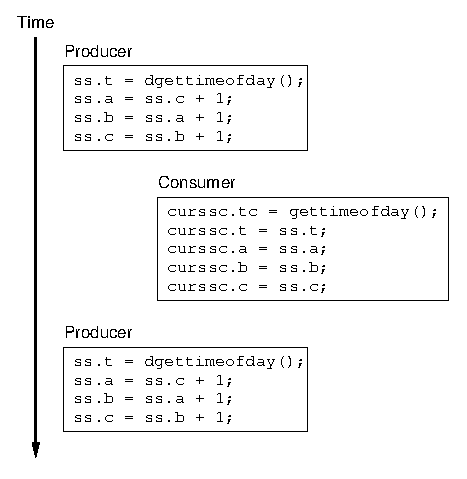
\includegraphics{appendix/questions/after}
\end{center}
\caption{Effect of Locking on Snapshot Collection}
\label{fig:app:questions:Effect of Locking on Snapshot Collection}
\end{figure}

This addition of locking results in output as shown in
Figure~\ref{fig:app:questions:Locked After Program Sample Output}.
Here there are no instances of time going backwards, instead,
there are only cases with more than 1,000 counts different between
consecutive reads by the consumer.

\begin{table}[htbp]
{ \scriptsize
\begin{tabular}{rcrrrr}
seq    & time (seconds) & delta~    &  a &  b &  c \\
\hline
58597:  & 1156521.556296 & (3.815) & 1485 & 1485 & 1485 \\
403927: & 1156523.446636 & (2.146) & 2583 & 2583 & 2583 \\
\end{tabular}
}
\caption{Locked ``After'' Program Sample Output}
\label{fig:app:questions:Locked After Program Sample Output}
\end{table}

\QuickQuiz{}
	How could there be such a large gap between successive
	consumer reads?
	See \url{timelocked.c} for full code.
\QuickQuizAnswer{
	\begin{enumerate}
	\item	The consumer might be preempted for long time periods.
	\item	A long-running interrupt might delay the consumer.
	\item	The producer might also be running on a faster CPU than is the
		consumer (for example, one of the CPUs might have had to
		decrease its
		clock frequency due to heat-dissipation or power-consumption
		constraints).
	\end{enumerate}
} \QuickQuizEnd

In summary, if you acquire an exclusive lock, you {\em know} that
anything you do while holding that lock will appear to happen after
anything done by any prior holder of that lock.
No need to worry about which CPU did or did not execute a memory
barrier, no need to worry about the CPU or compiler reordering
operations -- life is simple.
Of course, the fact that this locking prevents these two pieces of
code from running concurrently might limit the program's ability
to gain increased performance on multiprocessors, possibly resulting
in a ``safe but slow'' situation.
Chapter~\ref{cha:Partitioning and Synchronization Design} describes ways of
gaining performance and scalability in many situations.

However, in most cases, if you find yourself worrying about what happens
before or after a given piece of code, you should take this as a hint to
make better use of the standard primitives.
Let these primitives do the worrying for you.

% appendix/questions/concurrentparallel.tex
% SPDX-License-Identifier: CC-BY-SA-3.0

\section{What is the Difference Between ``Concurrent'' and ``Parallel''?}
\label{sec:app:questions:What is the Difference Between ``Concurrent'' and ``Parallel''?}

From a classic computing perspective, ``concurrent'' and ``parallel''
are clearly synonyms.
However, this has not stopped many people from drawing distinctions
between the two, and it turns out that these distinctions can be
understood from a couple of different perspectives.

The first perspective treats ``parallel'' as an abbreviation for
``data parallel'', and treats ``concurrent'' as pretty much everything
else.
From this perspective, in parallel computing, each partition of the
overall problem can proceed completely independently, with no
communication with other partitions.
In this case, little or no coordination among partitions is required.
In contrast, concurrent computing might well have tight interdependencies,
in the form of contended locks, transactions, or other synchronization
mechanisms.

\QuickQuiz{}
	Suppose a portion of a program uses RCU read-side primitives
	as its only synchronization mechanism.
	Is this parallelism or concurrency?
\QuickQuizAnswer{
	Yes.
} \QuickQuizEnd

This of course begs the question of why such a distinction matters,
which brings us to the second perspective, that of the underlying scheduler.
Schedulers come in a wide range of complexities and capabilities, and
as a rough rule of thumb, the more tightly and irregularly a set of
parallel processes communicate, the higher the level of sophistication
is required from the scheduler.
As such, parallel computing's avoidance of interdependencies means that
parallel-computing programs run well on the least-capable schedulers.
In fact, a pure parallel-computing program can run successfully after
being arbitrarily subdivided and interleaved onto a uniprocessor.\footnote{
	Yes, this does mean that parallel-computing programs are
	best-suited for sequential execution.
	Why did you ask?}
In contrast, concurrent-computing programs might well require extreme
subtlety on the part of the scheduler.

One could argue that we should simply demand a reasonable level of
competence from the scheduler, so that we could simply ignore any
distinctions between parallelism and concurrency.
Although this is often a good strategy,
there are important situations where efficiency,
performance, and scalability concerns sharply limit the level
of competence that the scheduler can reasonably offer.
One important example is when the scheduler is implemented in
hardware, as it often is in SIMD units or GPGPUs.
Another example is a workload where the units of work are quite
short, so that even a software-based scheduler must make hard choices
between subtlety on the one hand and efficiency on the other.

Now, this second perspective can be thought of as making the workload
match the available scheduler, with parallel workloads able to
operate on a simple scheduler and concurrent workloads requiring
more sophisticated schedulers.

Unfortunately, this perspective does not always align with the
dependency-based distinction put forth by the first perspective.
For example, a highly interdependent lock-based workload
with one thread per CPU can make do with a trivial scheduler
because no scheduler decisions are required.
In fact, some workloads of this type can even be run one after another
on a sequential machine.
Therefore, such a workload would be labeled ``concurrent'' by the first
perspective and ``parallel'' by many taking the second perspective.

\QuickQuiz{}
	In what part of the second (scheduler-based) perspective would
	the lock-based single-thread-per-CPU workload be considered
	``concurrent''?
\QuickQuizAnswer{
	The people who would like to arbitrarily subdivide and interleave
	the workload.
	Of course, an arbitrary subdivision might end up separating
	a lock acquisition from the corresponding lock release, which
	would prevent any other thread from acquiring that lock.
	If the locks were pure spinlocks, this could even result in
	deadlock.
} \QuickQuizEnd

Which is just fine.
No rule that humankind writes carries any weight against objective
reality, including the rule dividing multiprocessor programs into
categories such as ``concurrent'' and ``parallel''.

This categorization failure does not mean such rules are useless,
but rather that you should take on a suitably skeptical frame of mind when
attempting to apply them to new situations.
As always, use such rules where they apply and ignore them otherwise.

In fact, it is likely that new categories will arise in addition
to parallel, concurrent, map-reduce, task-based, and so on.
Some will stand the test of time, but good luck guessing which!

% appendix/questions/time.tex
% SPDX-License-Identifier: CC-BY-SA-3.0

\section{What Time Is It?}
\label{sec:app:questions:What Time Is It?}

\begin{figure}[htb]
\centering
\resizebox{3in}{!}{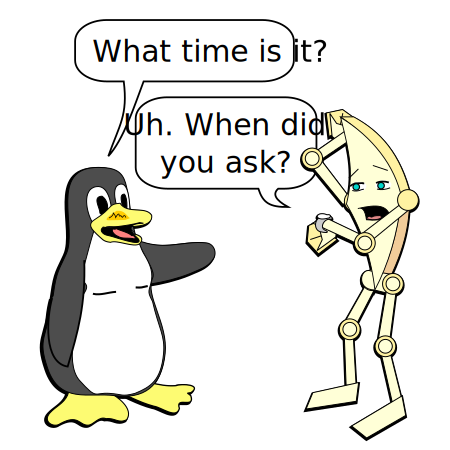
\includegraphics{cartoons/r-2014-What-time-is-it}}
\caption{What Time Is It?}
\ContributedBy{Figure}{fig:app:questions:What Time Is It?}{Melissa Broussard}
\end{figure}

A key issue with timekeeping on multicore computer systems is illustrated
by Figure~\ref{fig:app:questions:What Time Is It?}.
One problem is that it takes time to read out the time.
An instruction might read from a hardware clock, and might
have to go off-core (or worse yet, off-socket) to complete
this read operation.
It might also be necessary to do some computation on the value read out,
for example, to convert it to the desired format, to apply network time
protocol (NTP) adjustments, and so on.
So does the time eventually returned correspond to the beginning of
the resulting time interval, the end, or somewhere in between?

Worse yet, the thread reading the time might be interrupted or preempted.
Furthermore, there will likely be some computation between reading out
the time and the actual use of the time that has been read out.
Both of these possibilities further extend the interval of uncertainty.

One approach is to read the time twice, and take the arithmetic mean
of the two readings, perhaps one on each side of the operation being
timestamped.
The difference between the two readings is then a measure of uncertainty
of the time at which the intervening operation occurred.

Of course, in many cases, the exact time is not necessary.
For example, when printing the time for the benefit of a human user,
we can rely on slow human reflexes to render internal hardware and
software delays irrelevant.
Similarly, if a server needs to timestamp the response to a client, any
time between the reception of the request and the transmission of the
response will do equally well.

% @@@ Scheduling ticks

% @@@ Tickless operation

% @@@ Timers

% @@@ Current time, monotonic operation

% @@@ The many ways in which time can appear to go backwards

% @@@ Causality, the only real time in SMP (or distributed) systems

